%%%%%%%%%%%%%%%%%%%%%%%%%%%%%%%%%%%%%%%%%%%%%%%%%%%%%%%%%%%%%%%%%%%%%%%%%%%%%%%%%%%%%%%%%%%%%%%%
%
% CS484 Written Question Template
%
% Acknowledgements:
% The original code is written by Prof. James Tompkin (james_tompkin@brown.edu).
% The second version is revised by Prof. Min H. Kim (minhkim@kaist.ac.kr).
%
% This is a LaTeX document. LaTeX is a markup language for producing 
% documents. Your task is to fill out this document, then to compile 
% it into a PDF document. 
%
% 
% TO COMPILE:
% > pdflatex thisfile.tex
%
% If you do not have LaTeX and need a LaTeX distribution:
% - Personal laptops (all common OS): www.latex-project.org/get/
% - We recommend latex compiler miktex (https://miktex.org/) for windows,
%   macTex (http://www.tug.org/mactex/) for macOS users.
%   And TeXstudio(http://www.texstudio.org/) for latex editor.
%   You should install both compiler and editor for editing latex.
%   The another option is Overleaf (https://www.overleaf.com/) which is 
%   an online latex editor.
%
% If you need help with LaTeX, please come to office hours. 
% Or, there is plenty of help online:
% https://en.wikibooks.org/wiki/LaTeX
%
% Good luck!
% Min and the CS484 staff
%
%%%%%%%%%%%%%%%%%%%%%%%%%%%%%%%%%%%%%%%%%%%%%%%%%%%%%%%%%%%%%%%%%%%%%%%%%%%%%%%%%%%%%%%%%%%%%%%%
%
% How to include two graphics on the same line:
% 
% \includegraphics[width=0.49\linewidth]{yourgraphic1.png}
% \includegraphics[width=0.49\linewidth]{yourgraphic2.png}
%
% How to include equations:
%
% \begin{equation}
% y = mx+c
% \end{equation}
% 
%%%%%%%%%%%%%%%%%%%%%%%%%%%%%%%%%%%%%%%%%%%%%%%%%%%%%%%%%%%%%%%%%%%%%%%%%%%%%%%%%%%%%%%%%%%%%%%%

\documentclass[11pt]{article}

\usepackage[english]{babel}
\usepackage[utf8]{inputenc}
\usepackage[colorlinks = true,
            linkcolor = blue,
            urlcolor  = blue]{hyperref}
\usepackage[a4paper,margin=1.5in]{geometry}
\usepackage{stackengine,graphicx}
\usepackage{fancyhdr}
\setlength{\headheight}{15pt}
\usepackage{microtype}
\usepackage{times}
\usepackage{booktabs}

% From https://ctan.org/pkg/matlab-prettifier
\usepackage[numbered,framed]{matlab-prettifier}

\frenchspacing
\setlength{\parindent}{0cm} % Default is 15pt.
\setlength{\parskip}{0.3cm plus1mm minus1mm}

\pagestyle{fancy}
\fancyhf{}
\lhead{Homework Writeup}
\rhead{CS 484}
\rfoot{\thepage}

\date{}

\title{\vspace{-1cm}Homework 2 Writeup}


\begin{document}
\maketitle
\vspace{-3cm}
\thispagestyle{fancy}

\section*{Instructions}
\begin{itemize}
  \item Describe any interesting decisions you made to write your algorithm.
  \item Show and discuss the results of your algorithm.
  \item Feel free to include code snippets, images, and equations.
  \item Use as many pages as you need, but err on the short side If you feel you only need to write a short amount to meet the brief, th
  
  \item \textbf{Please make this document anonymous.}
\end{itemize}

\section*{Image Filtering}

For image filtering, without FFT-based convolution and with zero padding, I first checked the shape of given kernel. If it is not odd dimension, it raises error. Next step is padding the image. I added an option {\it zero\_pad=False} for the mode of pad. If it is false, the mode is reflect which makes it as cv2.BORDER\_REFLECT\_101. I divided cases for color image and grayscale image, as the number of channels is different.
 To perform convolution, I used the formula of $h[m, n] = \sum_{k, l} f[k, l][m - k, n - l]$ for not FFT-based convolution. For FFT-based convolution, $g\ast h = F^{-1}[F[g]F[h]]$ is used. Kernel needed to be zero padded for FFT, to become the same dimension of original image. After zero padding, I shifted the kernel so that the center of kernel get to the top left. 
 The result of image filtering is in Figure 1. 

	\begin{figure}[h]
		\centering
		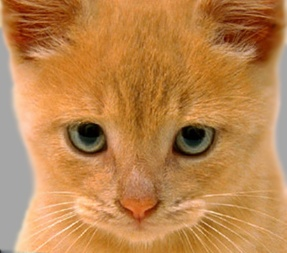
\includegraphics[width=5cm]{../result/test/identity_image.jpg}
		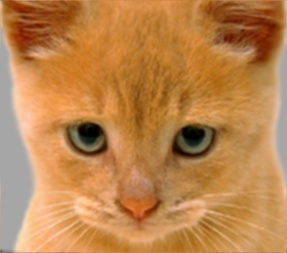
\includegraphics[width=5cm]{../result/test/blur_image.jpg}
		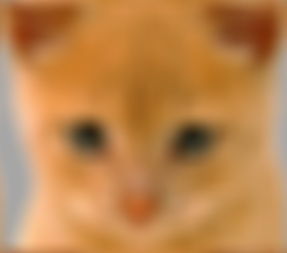
\includegraphics[width=5cm]{../result/test/large_blur_image.jpg}
		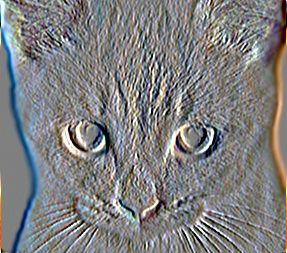
\includegraphics[width=5cm]{../result/test/sobel_image.jpg}
		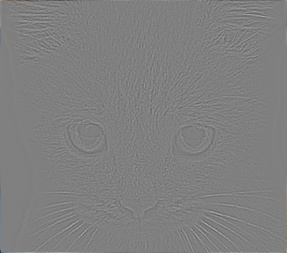
\includegraphics[width=5cm]{../result/test/high_pass_image.jpg}
		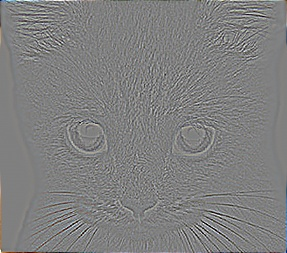
\includegraphics[width=5cm]{../result/test/laplacian_image.jpg}
		\caption{These are identity image, blur image, large blur image, sobel image, high pass image, and laplacian image from left to right, top to bottom. }
	\end{figure}

\section*{Hybrid Image}

To get the low frequency image, I used my my\_filter\_2D function using the given kernel. For high frequency image, I subtracted the low frequency image from original one. By adding the high and low frequency image, I got the hybrid image. The result is shown in Figure 2. 

	\begin{figure}[h]
		\centering
		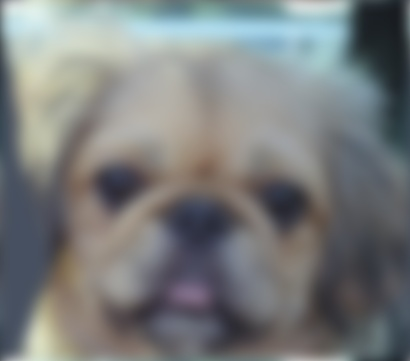
\includegraphics[width=5cm]{../result/low_frequencies.jpg}
		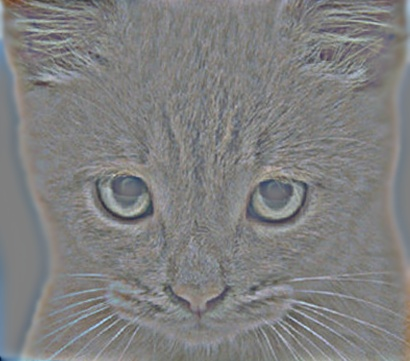
\includegraphics[width=5cm]{../result/high_frequencies.jpg}
		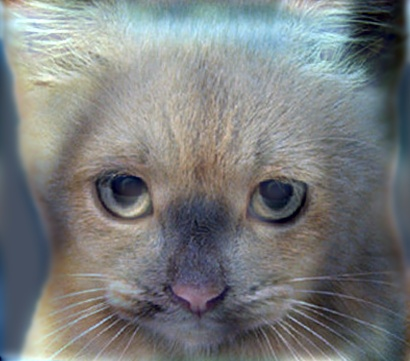
\includegraphics[width=5cm]{../result/hybrid_image.jpg}
		\caption{Hybrid image}
	\end{figure}


\end{document}
